\documentclass{article} 
\usepackage{geometry}
\geometry{legalpaper, portrait, margin=1in}
\usepackage{fancyhdr}
\usepackage{enumerate}
\usepackage{listings}
\usepackage{amsmath}
\usepackage{algorithm}
\usepackage{algpseudocode}
\usepackage{graphicx}
\usepackage{hyperref}
\usepackage{longtable}
\graphicspath{ }

\title{OpenFlow-based Adaptive Routing for Wireless Networks}
\author{
    Alok Kulkarni \\
    \textit{akulkar4@ncsu.edu}
    \and
    Angelyn Arputha Babu John \\
    \textit{ababujo@ncsu.edu}
    \and
    Jignesh Darji \\
    \textit{jndarji@ncsu.edu}
    \and 
    Nishad Sabnis \\
    \textit{nsabnis@ncsu.edu}
}
\date{
    \small{\url{https://sites.google.com/a/ncsu.edu/openflow-based-adaptive-routing-for-wireless-networks}}\\
    November 5th, 2015}

\pagestyle{fancy}
\fancyhf{}
\rhead{OpenFlow-based Adaptive Routing for Wireless Networks}
\lhead{CSC573}
\rfoot{Page \thepage}

\begin{document}
\maketitle
\section{Introduction}
\subsection{Problem Statement}
Designing a system to enable adaptive routing in a wireless network in order to make a comparative analysis of the
throughput efficiency of ground nodes versus aerial nodes.
\subsection{Problem Description}
\par We aim to implement OpenFlow based adaptive routing in an ad-hoc network by monitoring the link quality between wireless
nodes. We anticipate that in such a network which offers multiple wireless routes between two end-points, the
fluctuations in the RF link qualities between the endpoints will play an important role in determining the best end to
end path. Determining the wireless link quality between each and every inter-connected node and making routing decisions
based on this information constitute the two major parts of the problem. 
\par We plan to make aerial nodes a part of the network which will be used for testing. Aerial nodes have their own set of
advantages and disadvantages. They are less susceptible to electromagnetic interferences and can beam wifi over a large
area if the antennae are powerful enough. However, the number of aerial nodes and naturally the number of available
links through such nodes is likely to be lesser due to the low prevalence of such nodes. These trade offs need to be
accounted for while making the routing decisions as well. The final aim is to ensure that the flow tables are
dynamically modified to ensure effective end to end packet transmission. 
\section{Components}
\subsection{Platforms for the project}
\begin{itemize}
\item OpenFlow v1.3
\item Ubuntu
\item SDN Controller
\end{itemize}
\subsection{Areas for the project}
\begin{itemize}
\item Link Quality Monitoring
\item Adaptive Routing
\end{itemize}
\subsection{Major Components}
\subsubsection{Wireless Ground Nodes}
The ground nodes will be laptops. They will have the following features:
\begin{itemize}
\item At least one wireless interface
\item At least one interface to connect to the host
\item Open vSwitch module installed
\item One of the ground nodes will be the controller
\end{itemize}
\subsubsection{Aerial Nodes}
The aerial nodes will have the capacity to go up till 30 feet and beem signals from above. The key features of the
aerial nodes are:
\begin{itemize}
\item At least one wireless interface
\item BeagleBone black Linux boards
\item Open vSwitch kernel module installed
\end{itemize}
\subsubsection{Software Components}
The software components will help determine the link quality and the optimum path, and they will configure the network
with the optimal path.
\begin{itemize}
\item Link Quality Information module
\item OpenFlow Control module
\end{itemize}
\section{Design}
\subsection{Overview}
\begin{figure}[H]
\caption{Design Overview}
\centering
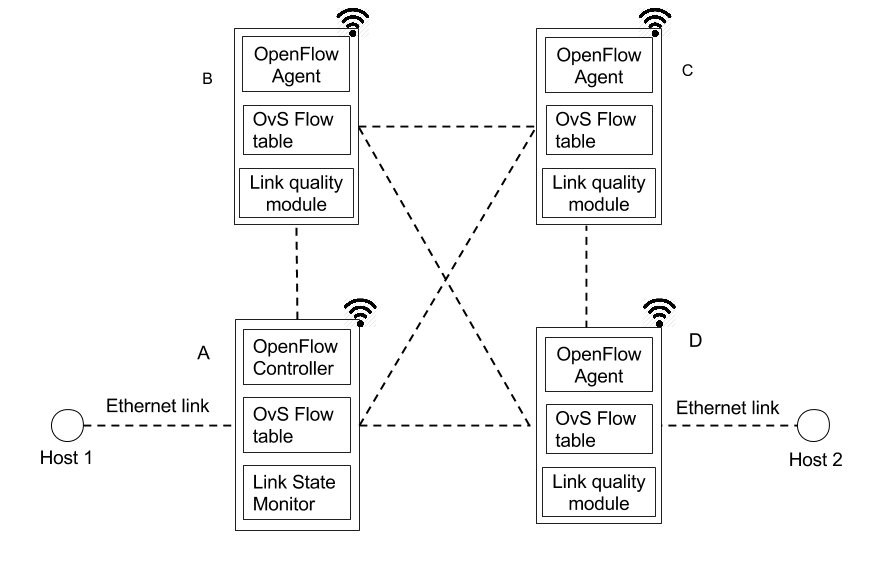
\includegraphics[width=\textwidth]{design}
\end{figure}
The above figure describes the overview of the components constituting this system. There exists a wireless ad-hoc
network of aerial and ground nodes. One of the nodes acts as an SDN controller and the others act as agents. A link
quality information (LQI) module is running on all the nodes in the network and this information is forwarded to the
OpenFlow controller which makes adaptive routing decisions. The controller will use this information to compute the
optimum end-to-end route between the endpoints. These routes will then be configured into the nodes using OpenFlow. The
nodes will have OVS running on them which will configure the routes sent by the Controller. 
\subsection{Link Quality Information Module}
\begin{figure}[H]
\caption{Components in the Link Quality Information Module}
\centering
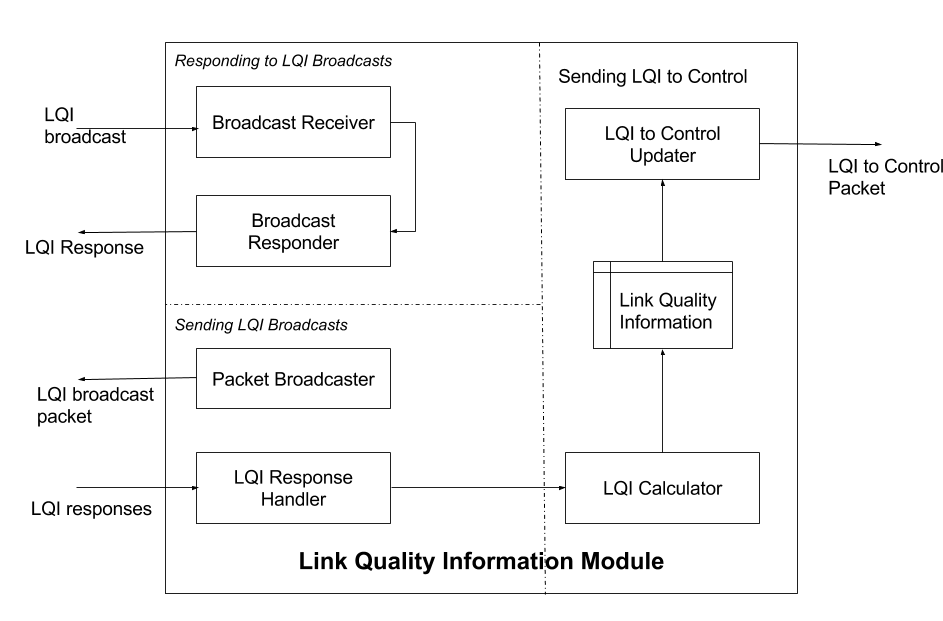
\includegraphics[width=\textwidth]{lqi}
\end{figure}
This module is responsible for estimating the point-to-point link quality between nodes. It will run on all the nodes in
the topology and give a periodically updated link quality estimate to the SDN controller. This information can then be
used by the SDN controller to update the topology and find the optimal path. The module is made up of two units: 
\begin{itemize}
\item \textit{Request unit}: It sends out the UDP broadcast and receives the responses for these broadcasts (Packet Broadcaster, Response Handler).
\item \textit{Response unit}: It receives the UDP broadcast and responds to it (Broadcast Receiver, Broadcast Responder).
\end{itemize}
\subsubsection{Packet Broadcaster} 
The LQI packet broadcaster will send out a UDP broadcast on the ad-hoc network. The broadcast is directed at a specific
UDP port to differentiate it from normal UDP traffic. The packet broadcaster will send out a broadcast packet after a 10
second interval. The UDP frame will look as follows:
%TODO: Add frame
\begin{figure}[H]
\centering
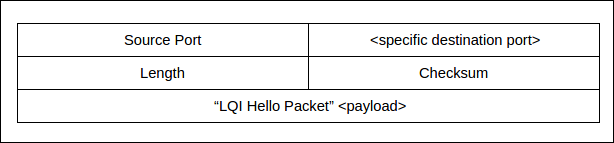
\includegraphics[width=\textwidth]{packet_broadcaster}
\end{figure}
\subsubsection{Broadcast Receiver}
Will listen on a specific port for LQI Hello packets and trigger the Broadcast Responder once it has verified the frame
format for each. 
\subsubsection{Broadcast Responder} 
Will prepare a unicast response for the broadcast source. The response will be sent out to a specific UDP port and will
have the following format. %TODO: Adding frame
\begin{figure}[H]
\centering
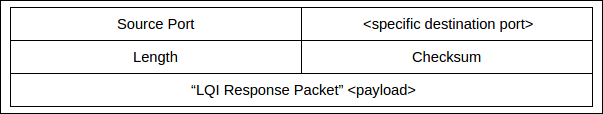
\includegraphics[width=\textwidth]{broadcast_responder}
\end{figure}
\subsubsection{Response Handler} 
The LQI Response Handler will listen at a specific port for any LQI responses, parse the LQI packet for obtaining the
SSI, source and destination IP and MAC, and forward the packet to the LQI calculator. The module will have a timeout
within which it expects to receive all the responses and will update the LQI Calculator after the timeout. The radiotap
header (LINKTYPE\_IEEE802\_11\_RADIOTAP) is an alternative to the normal 802.11 header (LINKTYPE\_IEEE802\_11) and and
contains some extra information about the wireless network along with the normal 802.11 header. The radiotap header
itself consists of a set of defined fields from which antenna signal (SSI) is to be extracted. The position of the
Radiotap header in the frame is as shown below. 
%TODO: Frame
\begin{figure}[H]
\centering
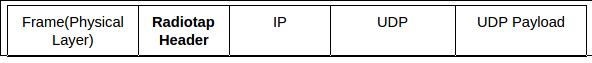
\includegraphics[width=\textwidth]{response_handler}
\end{figure}
\subsubsection{LQI Calculator} 
This module will get the SSI, source and destination IP and MAC address values from the Response Handler for all the
responses it receives. These value will be converted and stored in an LQI table in a format which can be further sent to
the controller.
\subsubsection{LQI to Control Updater} 
This module will refer to the values stored by the Calculator in LQI information table and prepare a payload that will
be sent to the controller. This packet will be used by the controller to create a topology and find the optimal path.
The format of the payload is as follows:
%TODO: Frame
\begin{figure}[H]
\centering
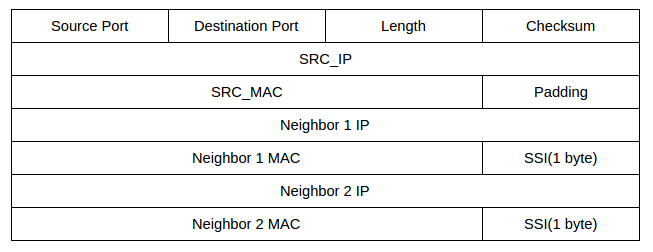
\includegraphics[width=\textwidth]{lqi_to_control_updater}
\end{figure}
\subsection{OpenFlow Control Module}
\begin{figure}[H]
\caption{Components in the OpenFlow Control application}
\centering
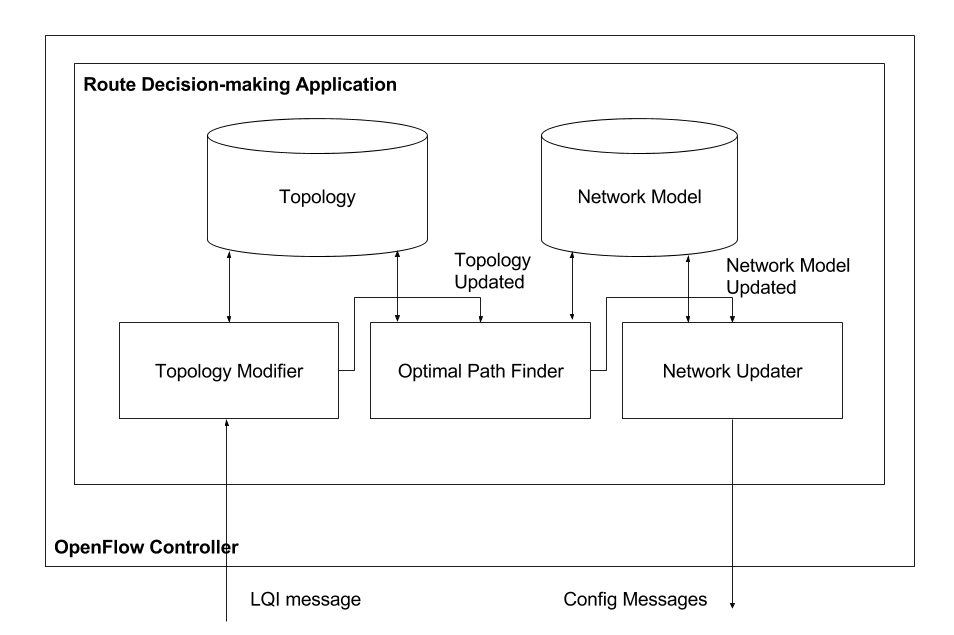
\includegraphics[width=\textwidth]{openflow}
\end{figure}
\subsubsection{Topology Modifier(TM)}
\textit{Function}: Generate and maintain the topology of the network and intimate Optimal Path Finder about topology change.
\begin{itemize}
\item Topology Construction: TM module accept the LQI messages and constructs the adjacency lists for all the nodes in
the network. The node data structure will contain following information be as follows:
\begin{itemize}
\item Node IP
\item Node MAC
\item Adjacent Nodes(IP and MAC) along with cost to reach them
\end{itemize}
\item \textit{Node Removal}: For each node, we shall have a running timer. If we do not get ‘N’ consecutive LQI messages from a
node, we shall remove the node from the topology. Calculation of N will be done later. We cannot have a high N because
the network convergence time would be affected. We cannot keep it low because that will mean a lot of reconfigurations
by the Network Updater if the node was not out of network or down but it’s LQI messages were dropped for a transient
duration due to other factors.
\item \textit{Topology Updates}: The TM module will be invoked to update the topology when one of the following event occurs in
the network:
\begin{itemize}
\item \textit{Node Addition}: When a node is added, it will be added to the adjacency list and cost to reach it from other nodes,
and costs from that new node to other nodes need to be updated.
\item \textit{Node Removal}: When a node is removed from the network(See “Node Removal” above), we need to remove its entry.
\item \textit{Cost Updates}: When the LQI message from a node is received with different costs, the adjacency list of that node
shall be update.
\end{itemize}
\item \textit{Callback to Optimal Path Finder}: When the topology is updated, it will send a callback to the OPF module.
\end{itemize}
\subsubsection{Optimal Path Finder(OPF)}
\textit{Function}: Find the lowest cost path between the end hosts.
\begin{itemize}
\item \textit{Limited Paths}: Since the topology is limited - 4 nodes and 2 of them connect to the end hosts - we have limited
end-to-end paths between the 2 edge nodes.
\begin{figure}[H]
\caption{Paths between edge nodes}
\centering
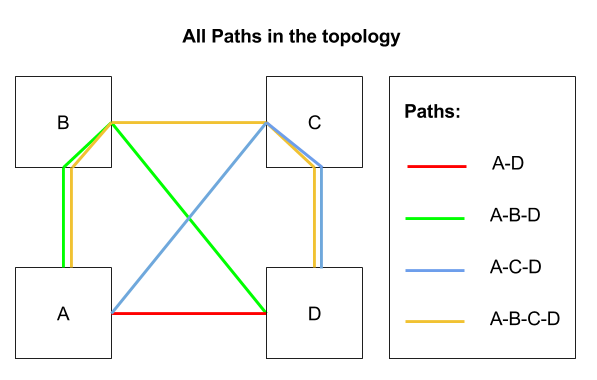
\includegraphics[width=\textwidth]{OPF_paths}
\end{figure}
\item \textit{Path Selection}: OPF will calculate path costs for all the 4 paths and select the least cost path.
\item \textit{Callback to Network Updater}: If the new path is different from the previous path, we send a callback to
the Network Updater.
\end{itemize}
\subsubsection{Network Updater(NU)}
\begin{itemize}
\item \textit{Problem}: Since the network is wireless ad-hoc and all the nodes can generally connect to each other, the
destination node will accept the packet directly. We need to enforce a method so that the packet follows the optimal
path calculated by the OPF and not the direct path between edge nodes.
\item \textit{Algorithm}: 
\begin{itemize}
\item \textit{Edge Nodes}: Install single rule on edge nodes to modify the DST\_MAC to it’s next node’s MAC. Here, next
node is the adjacent node in the optimal path.
\item \textit{Internal Nodes}: Install two rules on internal nodes to modify the DST\_MAC as well as SRC\_MAC for both the
directions. A simple illustration will clarify this step. 
\end{itemize}
\item \textit{Example}: In the below illustration, the edge nodes are A and D and the optimal path is A-B-D. To enforce
forwarding along A-\textgreater B-\textgreater D through the optimal path, A sends to B by changing the DST\_MAC to B’s MAC and then B sends to D
by changing the DST\_MAC to D’s MAC and SRC\_MAC to B’s MAC. Similar rules on D and B are required to enable for
D-\textgreater B-\textgreater A. 
\end{itemize}
\begin{figure}[H]
\caption{Flow Rule Illustration}
\centering
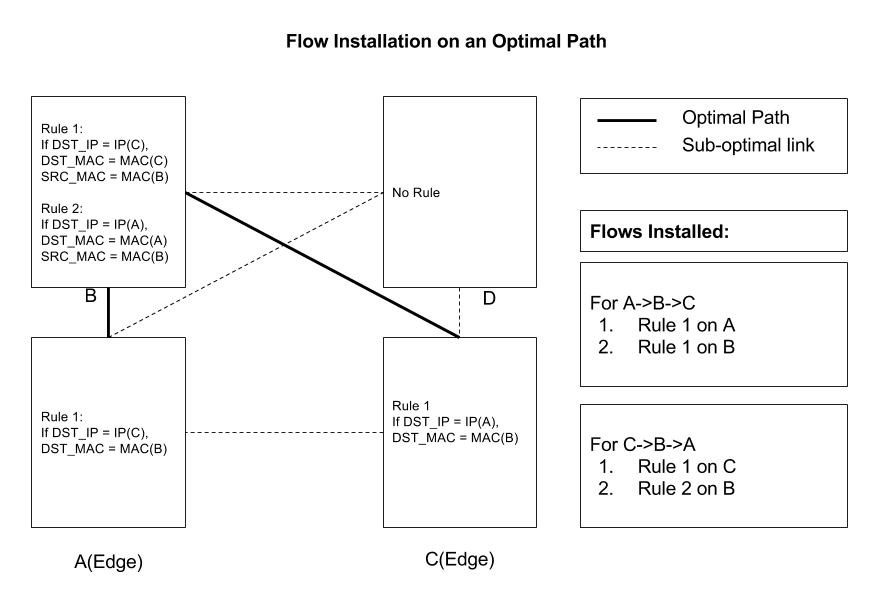
\includegraphics[width=\textwidth]{NU_Algorithm_Example}
\end{figure}

\section{Per-member Responsibilities}
{\renewcommand{\arraystretch}{1.5}
\begin{tabular}{ | p{0.185\linewidth} | p{0.185\linewidth} | p{0.185\linewidth} | p{0.185\linewidth} | p{0.185\linewidth} | }
\hline
\textbf{Tasks}	&	\textbf{Angelyn Arputha Babu John}	&	\textbf{Jignesh Darji}	&	\textbf{Nishad Sabnis}	& \textbf{Alok Kulkarni} \\
\hline \hline
Node Setup	&	Implement	&	Implement	&	Implement	&	Implement \\
\hline
Creation of ad-hoc network	&	Review	&	Review	&	Implement	&	Implement \\
\hline
LQI Message Handling	&	Review	&	Review	&	Implement	&	Implement \\ 
\hline
LQI Calculator	&	Review	&	Review	&	Review	&	Implement\\ 
\hline
LQI to Control Updater	&	Review	&	Review	&	Implement	&	Review \\
\hline
Topology Modifier	&	Implement	&	Implement	&	Review	&	Review\\
\hline
Optimal Path Finder	&	Implement	&	Implement	&	Review	&	Review\\
\hline
Network Updater	&	Implement	&	Implement	&	Review	&	Review\\
\hline
\end{tabular}}

\newpage
\section{Test Plan}
{\renewcommand{\arraystretch}{1.5}
\begin{longtable}{  | p{0.1\linewidth} | p{0.2\linewidth} | p{0.35\linewidth} | p{0.2\linewidth} | p{0.1\linewidth} | }
\hline
\textbf{Test ID} & \textbf{Test} & \textbf{Expected Observation} & \textbf{Conclusion} & \textbf{Result} \\ 
\hline \hline
T-1 & Establishing the ad-hoc Network & All the nodes (ground and aerial) are able to ping each other within the network
& Each node is able to join the ad-hoc network successfully & Pass \\
\hline
T-2 & 
Add a node with low path cost & 
\textbf{LQI Module}: Connected nodes transmit their respective costs with new node to LQI messages \newline 
\textbf{Topology Modifier}: Adds the node to the Topology; Intimate OPF \newline 
\textbf{Optimal Path Finder}: Adds the path to Network Model; Intimate NU \newline
\textbf{Network Updater}: Updates the affected nodes. &
The message packets are now sent through the path with least cost instead of following the costlier route &
Pass \\
\hline
T-3 & 
Add a node with high path cost & 
\textbf{LQI Module}: Connected nodes should transmit cost with the new node to the LQI messages\newline 
\textbf{Topology Modifier}: Add node to Topology; intimate OPF\newline 
\textbf{Optimal Path Finder}: Network Model remains same\newline
\textbf{Network Updater}: Not Affected &
The message is sent through the usual path and is not changed by the addition of this new node &
Pass\\
\hline
T-4 & 
Remove node from Network Model & 
\textbf{LQI Module}: LQI messages will not contain costs to this node\newline 
\textbf{Topology Modifier}: Remove node from Topology; intimate OPF \newline 
\textbf{Optimal Path Finder}: Modifies Network Model; intimate NU \newline
\textbf{Network Updater}: Updates the affected nodes &
The node is successfully removed from the topology with or without affecting the other nodes &
Pending\\
\hline
T-5 & 
Remove node not part of the Network Model & 
\textbf{LQI Module}: LQI messages will not contain costs to this node\newline 
\textbf{Topology Modifier}: Remove node from Topology; intimate OPF\newline 
\textbf{Optimal Path Finder}: Modifies Network Model; intimate NU\newline
\textbf{Network Updater}: Not Affected &
The controller ignores this change as it is not part of the network &
Pending\\
\hline
T-6 & 
Increase associated path cost of a node in Network Model & 
\textbf{LQI Module}:  Cost to this node should be increased in the LQI messages\newline 
\textbf{Topology Modifier}: Update path costs in Topology; intimate OPF\newline 
\textbf{Optimal Path Finder}: Modifies Network Model; intimate NU\newline
\textbf{Network Updater}: Update the affected nodes &
Changes in the network are noticed as the controller routes the packet through the cheaper route &
Pending\\
\hline
T-7 & 
Increase associated path cost of a node NOT in the Network Model & 
\textbf{LQI Module}: Cost to this node should be increased in the LQI messages\newline 
\textbf{Topology Modifier}: Update path costs in Topology; intimate OPF\newline 
\textbf{Optimal Path Finder}: Network Model remains unchanged\newline
\textbf{Network Updater}: Not affected &
The controller ignores this change as it is not part of the network &
Pending\\
\hline
T-8 & 
Decrease associated path cost of a node in Network Model & 
\textbf{LQI Module}: Cost to this node should be decreased in the LQI messages\newline 
\textbf{Topology Modifier}: Update path costs in Topology; intimate OPF \newline 
\textbf{Optimal Path Finder}: Modifies Network Model; intimate NU\newline
\textbf{Network Updater}: Update the affected nodes \newline &
The network changes as the controller routes the packet through the newest path with least cost. &
Pending\\
\hline
T-9 & 
Decrease associated path cost of a node NOT in the Network Model & 
\textbf{LQI Module}: Cost to this node should be increased in the LQI messages\newline 
\textbf{Topology Modifier}: Update path costs in Topology; intimate OPF\newline 
\textbf{Optimal Path Finder}: Network Model remains unchanged\newline
\textbf{Network Updater}: Not affected &
The controller ignores this change as it is not part of the network &
Pending\\
\hline
\end{longtable}}
\section{Demo Plan}
{\renewcommand{\arraystretch}{1.5}
\begin{tabular}{ | p{0.095\linewidth} | p{0.285\linewidth} | p{0.285\linewidth} | p{0.285\linewidth} | }
\hline
\textbf{Demo ID}	&	\textbf{Scenario}	&	\textbf{Expected Observation}	&	\textbf{Conclusion}	\\ 
\hline \hline
D-1 & The nodes will be arranged such that the shortest path from A to D is A-\textgreater D. Then a simple data stream from Host 1
to Host 2 will be started. Tcpdump will be running on all nodes & Tcpdump for A and D nodes will show the data stream
but tcpdump for B and C nodes will show no activity & The system has setup the flow in such a way that the route is
direct. \\
\hline
D-2 & The nodes will be arranged such that the shortest path from A to D is A-\textgreater B-\textgreater C-\textgreater D. Then a simple data stream from
Host 1 to Host 2 will be started. Tcpdump will be running on all nodes & Tcpdump for A,B,C,D nodes will show the data
stream and indicate the packet path & The system has setup the flow in such a way that the route is not the direct
route. LQI based routing has successfully taken place and routes have been configured accordingly \\
\hline
\end{tabular}}
\section{Self-study Plan}
\subsection{Description of Base Case}
The base case for our system is a 4 node wireless ad-hoc network topology. In a normal ad-hoc topology, if a
transmission has to be sent from node A to node D, it will be sent directly(A-\textgreater D). This takes place irrespective of the
link quality between these nodes as these nodes are in the same wireless ad-hoc network. Also, it is to be noted that in
case A and D are not in range of each other, the transmission is not possible.
\subsection{Characteristics to Observe}
The main characteristics to observe in this case are as follows:
\begin{enumerate}
\item \textit{Link quality}: The wireless link quality between each and every node is an important characteristic which will be
continuously observed and reported as mentioned above. 
\item \textit{Packet path}: The packet path will adhere to the rules set by the SDN controller. A method to observe the path has
been discussed in the test cases above. 
\item \textit{Latency}: The latency when the packet goes normally(as in base case) from A-\textgreater D and when it takes a different route
will be indicative of the tradeoffs between time-delay and link quality. The measurements will be recorded in log files
so that they can be reviewed.
\end{enumerate}
\subsection{Range of Scenarios to Investigate}
There will be three major scenarios to investigate in this system are as follows:
\begin{enumerate}
\item The first scenario will be to observe edge-to-edge packet forwarding without any OpenFlow flows installed. It is
expected that a packet destined to reach router D from router A, will be sent directly to router D. The main things
which will be important to observe and consider is the time delay that it takes for this transmission, successful
delivery of packet to D and the link quality between A and D. 
\item The second scenario will be set up in such a way that the OpenFlow Flow tables are setup as mentioned in the
low-level design and edge-to-edge forwarding is carried out. In this scenario it is expected that, the link quality
between A- \textgreater D be lower than the link qualities between B-\textgreater D and A-\textgreater B.  The packet
will then take the path A-\textgreater B-\textgreater D and the
timing delay will be observed. We think that the packet will take more time as it is coming via a longer route in spite
of a shorter route with poorer link quality being available.
\item In the third scenario, we will set up the network so that A and D are not in range. In this case it is expected
that the base case will fail to transmit but the proposed system shall deliver the packet successfully albeit with a
higher delay.  
\end{enumerate}
\begin{thebibliography}{5}
\bibitem{openflow}
OpenFlow Switch Specification
\\\texttt{http://archive.openflow.org/documents/openflow-wp-latest.pdf}
\bibitem{rfc2501}
RFC 2501: Wireless ad-hoc Networks
\\\texttt{https://tools.ietf.org/html/rfc2501}
\bibitem{tcpdump}
Radiotap header
\\\texttt{http://www.radiotap.org/}
\bibitem{}
Open VSwitch
\\\texttt{http://openvswitch.org/}
\bibitem{}
RFC 768: User Datagram Protocol
\\\texttt{https://www.ietf.org/rfc/rfc768.txt}
\bibitem{}
\textit{tcpdump} utility
\\\texttt{http://www.tcpdump.org/}
\bibitem{}
\textit{libpcap} library
\\\texttt{http://www.tcpdump.org/}
\end{thebibliography}
\end{document}
